\documentclass[,man]{apa6}
\usepackage{lmodern}
\usepackage{amssymb,amsmath}
\usepackage{ifxetex,ifluatex}
\usepackage{fixltx2e} % provides \textsubscript
\ifnum 0\ifxetex 1\fi\ifluatex 1\fi=0 % if pdftex
  \usepackage[T1]{fontenc}
  \usepackage[utf8]{inputenc}
\else % if luatex or xelatex
  \ifxetex
    \usepackage{mathspec}
  \else
    \usepackage{fontspec}
  \fi
  \defaultfontfeatures{Ligatures=TeX,Scale=MatchLowercase}
\fi
% use upquote if available, for straight quotes in verbatim environments
\IfFileExists{upquote.sty}{\usepackage{upquote}}{}
% use microtype if available
\IfFileExists{microtype.sty}{%
\usepackage{microtype}
\UseMicrotypeSet[protrusion]{basicmath} % disable protrusion for tt fonts
}{}
\usepackage{hyperref}
\hypersetup{unicode=true,
            pdftitle={Relations between early entrance to childcare and infant intestinal microbiota},
            pdfauthor={Henrik Eckermann, Gerben Hermes, \& Carolina de Weerth},
            pdfkeywords={microbiota, childcare, breastfeeding, early life stress},
            pdfborder={0 0 0},
            breaklinks=true}
\urlstyle{same}  % don't use monospace font for urls
\usepackage{graphicx,grffile}
\makeatletter
\def\maxwidth{\ifdim\Gin@nat@width>\linewidth\linewidth\else\Gin@nat@width\fi}
\def\maxheight{\ifdim\Gin@nat@height>\textheight\textheight\else\Gin@nat@height\fi}
\makeatother
% Scale images if necessary, so that they will not overflow the page
% margins by default, and it is still possible to overwrite the defaults
% using explicit options in \includegraphics[width, height, ...]{}
\setkeys{Gin}{width=\maxwidth,height=\maxheight,keepaspectratio}
\IfFileExists{parskip.sty}{%
\usepackage{parskip}
}{% else
\setlength{\parindent}{0pt}
\setlength{\parskip}{6pt plus 2pt minus 1pt}
}
\setlength{\emergencystretch}{3em}  % prevent overfull lines
\providecommand{\tightlist}{%
  \setlength{\itemsep}{0pt}\setlength{\parskip}{0pt}}
\setcounter{secnumdepth}{0}
% Redefines (sub)paragraphs to behave more like sections
\ifx\paragraph\undefined\else
\let\oldparagraph\paragraph
\renewcommand{\paragraph}[1]{\oldparagraph{#1}\mbox{}}
\fi
\ifx\subparagraph\undefined\else
\let\oldsubparagraph\subparagraph
\renewcommand{\subparagraph}[1]{\oldsubparagraph{#1}\mbox{}}
\fi

%%% Use protect on footnotes to avoid problems with footnotes in titles
\let\rmarkdownfootnote\footnote%
\def\footnote{\protect\rmarkdownfootnote}


  \title{Relations between early entrance to childcare and infant intestinal
microbiota}
    \author{Henrik Eckermann\textsuperscript{1}, Gerben Hermes\textsuperscript{2},
\& Carolina de Weerth\textsuperscript{1}}
    \date{}
  
\shorttitle{Relations between early entrance to childcare and infant intestinal microbiota}
\affiliation{
\vspace{0.5cm}
\textsuperscript{1} Radboud University Nijmegen\\\textsuperscript{2} Wageningen University}
\keywords{microbiota, childcare, breastfeeding, early life stress\newline\indent Word count: 138}
\usepackage{csquotes}
\usepackage{upgreek}
\captionsetup{font=singlespacing,justification=justified}

\usepackage{longtable}
\usepackage{lscape}
\usepackage{multirow}
\usepackage{tabularx}
\usepackage[flushleft]{threeparttable}
\usepackage{threeparttablex}

\newenvironment{lltable}{\begin{landscape}\begin{center}\begin{ThreePartTable}}{\end{ThreePartTable}\end{center}\end{landscape}}

\makeatletter
\newcommand\LastLTentrywidth{1em}
\newlength\longtablewidth
\setlength{\longtablewidth}{1in}
\newcommand{\getlongtablewidth}{\begingroup \ifcsname LT@\roman{LT@tables}\endcsname \global\longtablewidth=0pt \renewcommand{\LT@entry}[2]{\global\advance\longtablewidth by ##2\relax\gdef\LastLTentrywidth{##2}}\@nameuse{LT@\roman{LT@tables}} \fi \endgroup}


\DeclareDelayedFloatFlavor{ThreePartTable}{table}
\DeclareDelayedFloatFlavor{lltable}{table}
\DeclareDelayedFloatFlavor*{longtable}{table}
\makeatletter
\renewcommand{\efloat@iwrite}[1]{\immediate\expandafter\protected@write\csname efloat@post#1\endcsname{}}
\makeatother
\usepackage[titles]{tocloft}
\cftpagenumbersoff{figure}
\renewcommand{\cftfigpresnum}{\itshape\figurename\enspace}
\renewcommand{\cftfigaftersnum}{.\space}
\setlength{\cftfigindent}{0pt}
\setlength{\cftafterloftitleskip}{0pt}
\settowidth{\cftfignumwidth}{Figure 10.\qquad}
\cftpagenumbersoff{table}
\renewcommand{\cfttabpresnum}{\itshape\tablename\enspace}
\renewcommand{\cfttabaftersnum}{.\space}
\setlength{\cfttabindent}{0pt}
\setlength{\cftafterloftitleskip}{0pt}
\settowidth{\cfttabnumwidth}{Table 10.\qquad}

\authornote{

Correspondence concerning this article should be addressed to Henrik
Eckermann, Kreuzfurth 10, 47559 Kranenburg, Germany. E-mail:
\href{mailto:h.eckermann@student.ru.nl}{\nolinkurl{h.eckermann@student.ru.nl}}}

\abstract{
Attending center based childcare (CC) at three months of life can be an
important life changing event that includes major stressors such as long
maternal separations and frequently changing caregivers. These in turn
may alter the composition of the gut microbiota with possible
implications for future health outcomes. As part of an ongoing
longitudinal study, we investigated whether CC compared to being cared
by the mother at home alters the composition of the gut microbiota and
whether breastfeeding buffers the potential effect of CC on the
microbiota. Stool samples of infants who entered CC (n=49) and control
infants (n=49) were obtained before and four weeks after CC entrance. We
did not observe an effect of CC on overall community composition.
Infants who entered CC had lower alpha diversity post CC compared to no
CC or pre CC.


}

\begin{document}
\maketitle

\section{3. Results}\label{results}

\subsection{3.1. Microbiota composition}\label{microbiota-composition}

Thirteen genus like groups from the \emph{Actinobacteria},
\emph{Firmicutes}, \emph{Proteobacteria} and phyla showed an average
abundance of \(\geq 0.05\) \% in at least 20\% of the samples (Figure
1). Overall the microbiota was dominated by \emph{Bifidobacterium} with
an average abundance of more than 50\%. Followed by facultative
anaerobic \emph{Bacilli} (\emph{Streptococcus spp}, \emph{Enterococcus},
\emph{Lactobacilllus} and \emph{Granulicatella}). The general variation
of relative abundance of all taxa was quite high, with
\emph{Bifidobacterium} for instance ranging from 0.2\% to 89\%.

Figure 2 shows microbiota composition (Aitchison distance) for the first
four principal components within the CC (A) and within the HOME (B)
group. The starting points of the arrows indicate the microbiota
composition in space at PRE, whereas the endpoint corresponds the
composition at POST. There appear to be no differences in in location
between CC and HOME at PRE or POST. Also we did not identify a uniform
direction of the shifts over time in either group. Instead, microbiota
composition development between time points appears to be highly
individual.

\begin{figure}
\centering
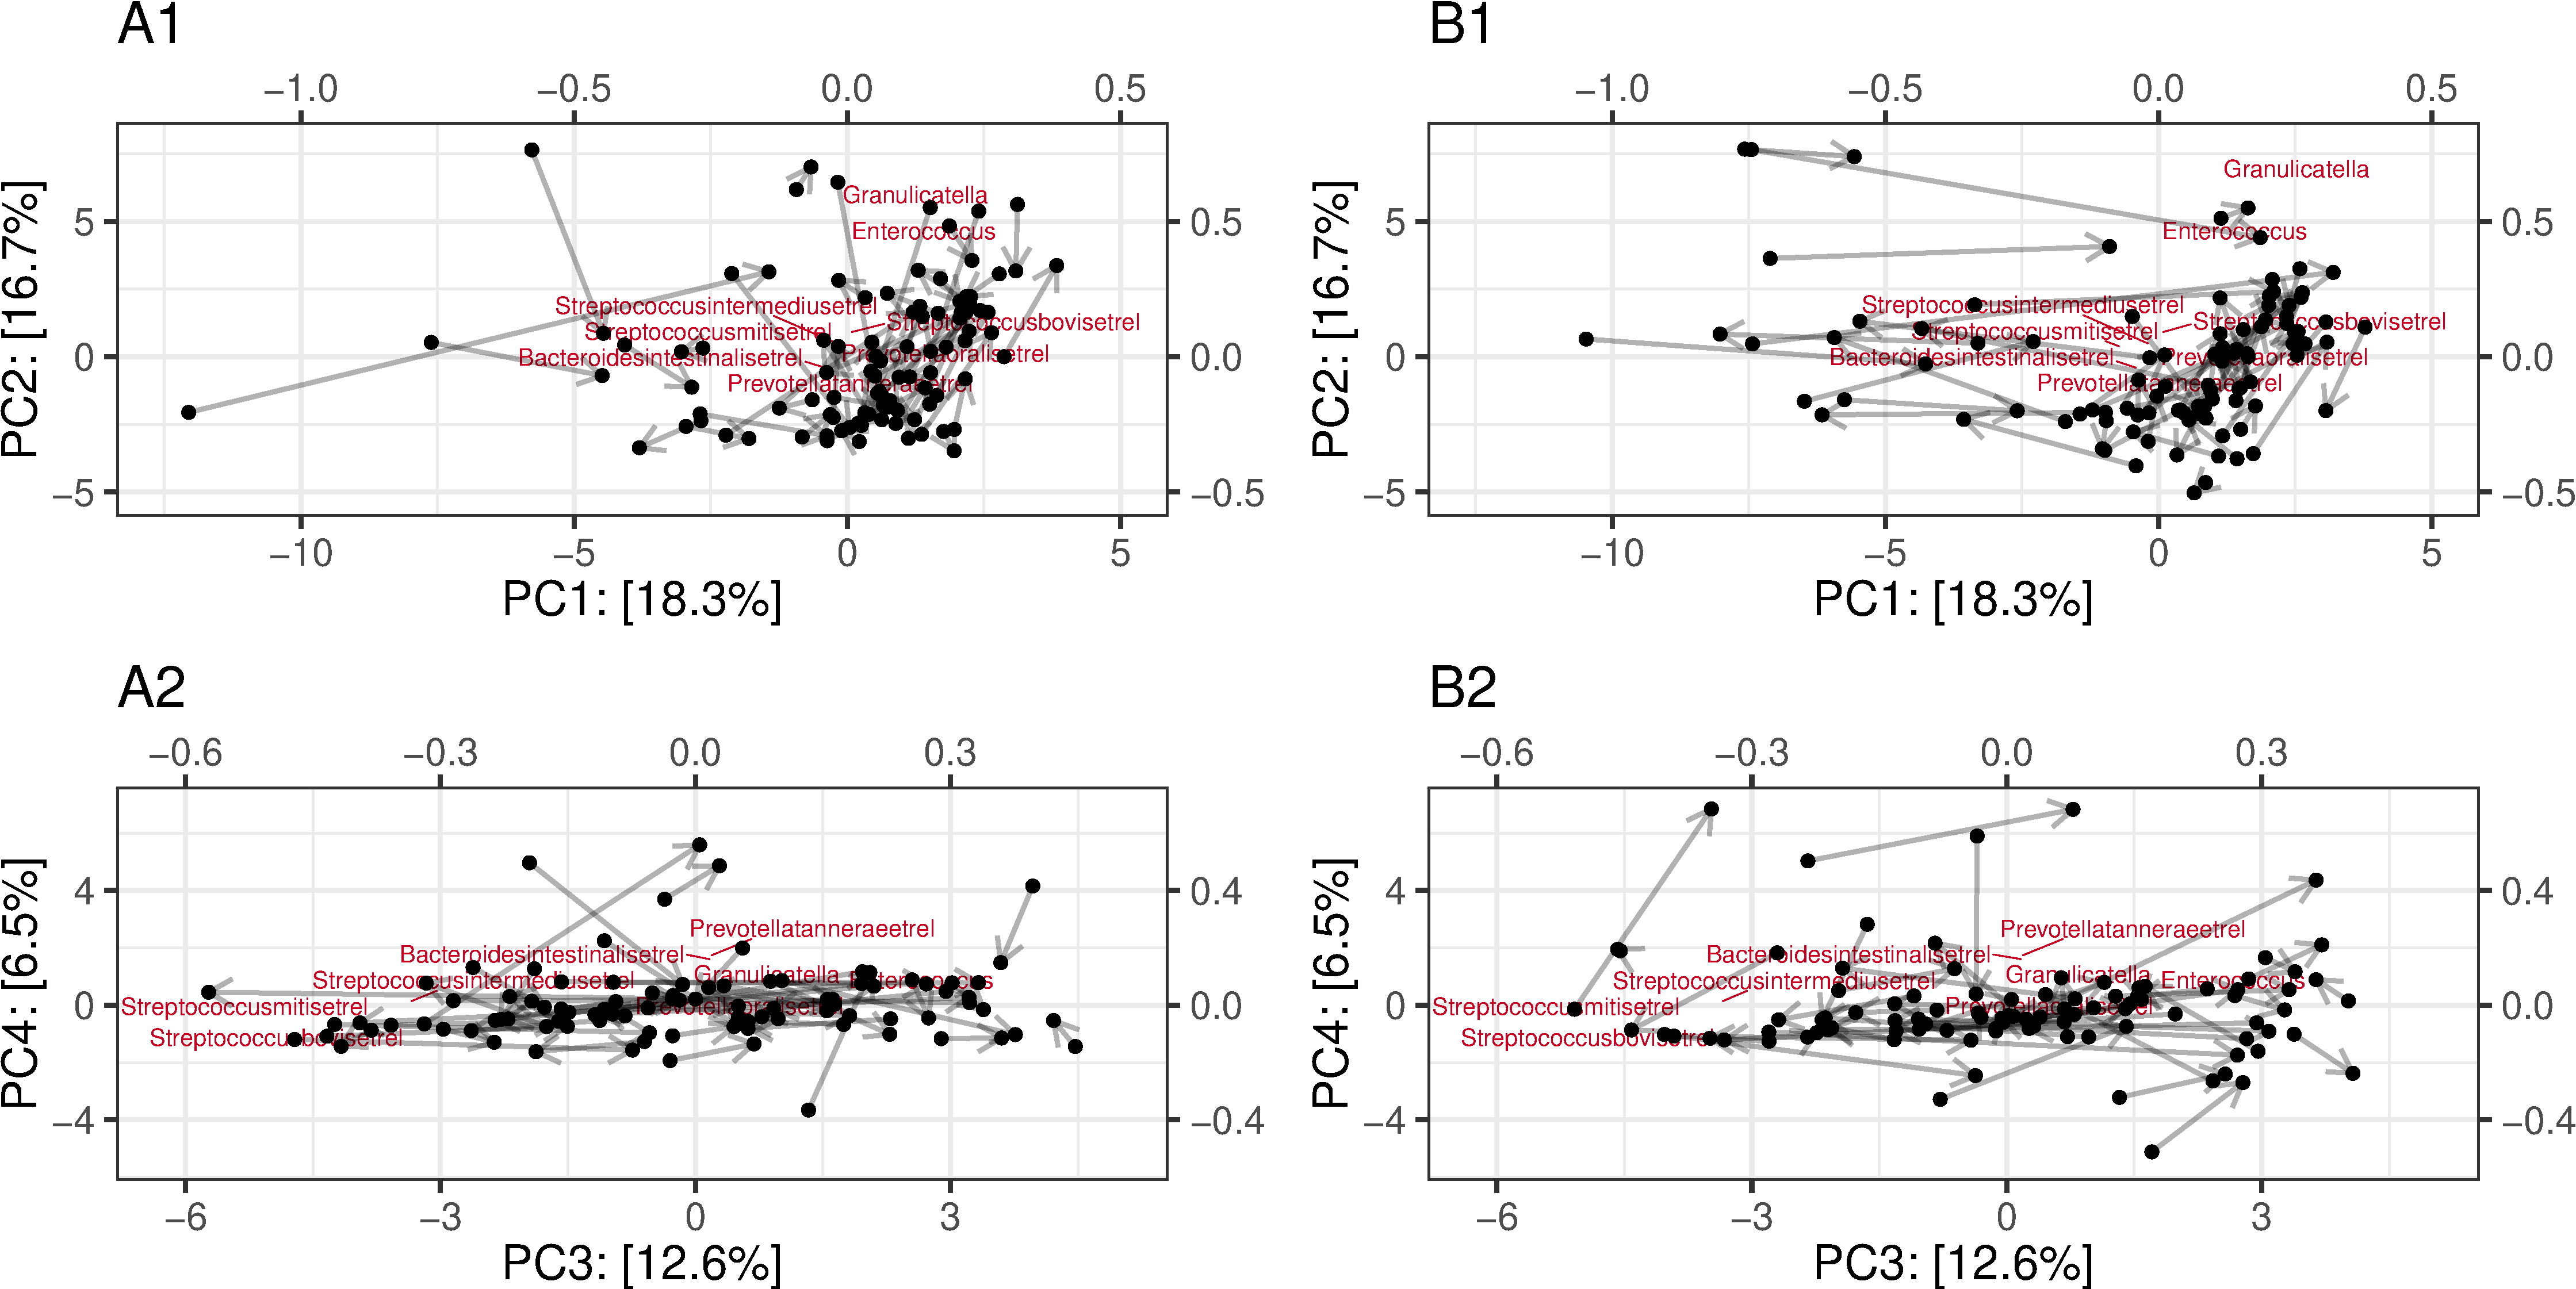
\includegraphics{index_files/figure-latex/unnamed-chunk-7-1.pdf}
\caption{\label{fig:unnamed-chunk-7}Development of microbiota composition
over time within CC (A and C) and no CC (B and D).}
\end{figure}

\subsection{3.2 Effects of CC on microbiota
composition}\label{effects-of-cc-on-microbiota-composition}

We used age and the average number of breast-feedings per day as
covariates in all linear models. Table 1 shows these and other variables
for both groups. There was a significant difference in age between
groups \emph{t}(62.42) = -4.54, \emph{p} \textless{} .001 according to
Welch's t-test. Besides that, there were no differences between groups
for any of the remaining variables.

\begin{table}[tbp]
\begin{center}
\begin{threeparttable}
\caption{\label{tab:unnamed-chunk-8}Descriptive statistics for demographic variables of infants and mothers included in the present study.}
\begin{tabular}{lll}
\toprule
 & \multicolumn{1}{c}{CC (n = 49)} & \multicolumn{1}{c}{HOME (n = 49)}\\
\midrule
**Gender** &  & \\
\ \ \ male & 29 & 25\\
\ \ \ female & 20 & 24\\
**Age (weeks)** &  & \\
\ \ \ mean (sd) & 12.8 $\pm$ 2.3 & 11.2 $\pm$ 0.9\\
\ \ \ min & 8.6 & 10.0\\
\ \ \ max & 17.9 & 13.1\\
**Maternal Education** &  & \\
\ \ \ mean (sd) & 32.9 $\pm$ 3.0 & 32.2 $\pm$ 3.6\\
\ \ \ min & 25.1 & 24.9\\
\ \ \ max & 42.0 & 40.1\\
**Birthweight** &  & \\
\ \ \ mean (sd) & 3630.4 $\pm$ 508.9 & 3636.0 $\pm$ 438.4\\
\ \ \ min & 2708 & 2810\\
\ \ \ max & 4600 & 4700\\
**Breastfeeding (Birth - PRE)** &  & \\
\ \ \ mean (sd) & 5.1 $\pm$ 2.9 & 6.0 $\pm$ 2.2\\
\ \ \ min & 0 & 0\\
\ \ \ max & 8.9 & 11.4\\
**Breastfeeding (PRE - POST)** &  & \\
\ \ \ mean (sd) & 4.0 $\pm$ 2.8 & 3.8 $\pm$ 3.0\\
\ \ \ min & 0 & 0\\
\ \ \ max & 8.5 & 8.5\\
\bottomrule
\addlinespace
\end{tabular}
\begin{tablenotes}[para]
\normalsize{\textit{Note.} CC = childcare. Breastfeeding refers to the average number of breast-feedings per day.}
\end{tablenotes}
\end{threeparttable}
\end{center}
\end{table}

\subsection{3.2.1 Permutational multivariate
ANOVA}\label{permutational-multivariate-anova}

We compared the overall community composition using PERMANOVA based on
Aitchison distance metric. An assumption for PERMANOVA is multivariate
homogeneity of group dispersions (variances) ({\textbf{???}}). We used
the function \emph{betadisper} ({\textbf{???}}), which utilizes the
\emph{PERMDISP2} procedure as implemented by Marti Anderson and found
that this assumption was met for the factors \emph{childcare}
\emph{F}(1,194) = 0.19, \emph{p} = .188, \emph{time} \emph{F}(1,194) =
1.73, \emph{p} = .190 and the subgroups that result out of the
interaction of \emph{time} and \emph{cc} \emph{F}(3,192) = 1.19,
\emph{p} = .313. We did not find a significant effect of CC over time on
overall community composition (see table x). Breastfeeding and age
significantly predicted overall community composition. Figure x shows
the genera that mostly changed as a function of each significant
predictor.

\begin{table}[tbp]
\begin{center}
\begin{threeparttable}
\caption{\label{tab:unnamed-chunk-9}Table x. Model Output PERMANOVA}
\begin{tabular}{lllllll}
\toprule
Model Parameter & \multicolumn{1}{c}{Sum of Squares} & \multicolumn{1}{c}{Mean Sum of Squares} & \multicolumn{1}{c}{F} & \multicolumn{1}{c}{Df} & \multicolumn{1}{c}{p} & \multicolumn{1}{c}{R Square}\\
\midrule
time & 58.44 & 58.444 & 1.469 & 1.00 & 0.118 & 0.01\\
cc & 52.64 & 52.636 & 1.323 & 1.00 & 0.192 & 0.01\\
age\_d\_s & 79.55 & 79.553 & 2 & 1.00 & 0.023 & 0.01\\
bf\_count\_s & 197.06 & 197.06 & 4.954 & 1.00 & 0.001 & 0.02\\
time:cc & 36.23 & 36.229 & 0.911 & 1.00 & 0.506 & 0.00\\
Residuals & 7,558.55 & 39.782 & - & 190.00 & - & 0.95\\
Total & 7,982.47 & - & - & 195.00 & - & 1.00\\
\bottomrule
\end{tabular}
\end{threeparttable}
\end{center}
\end{table}

\begin{figure}
\centering
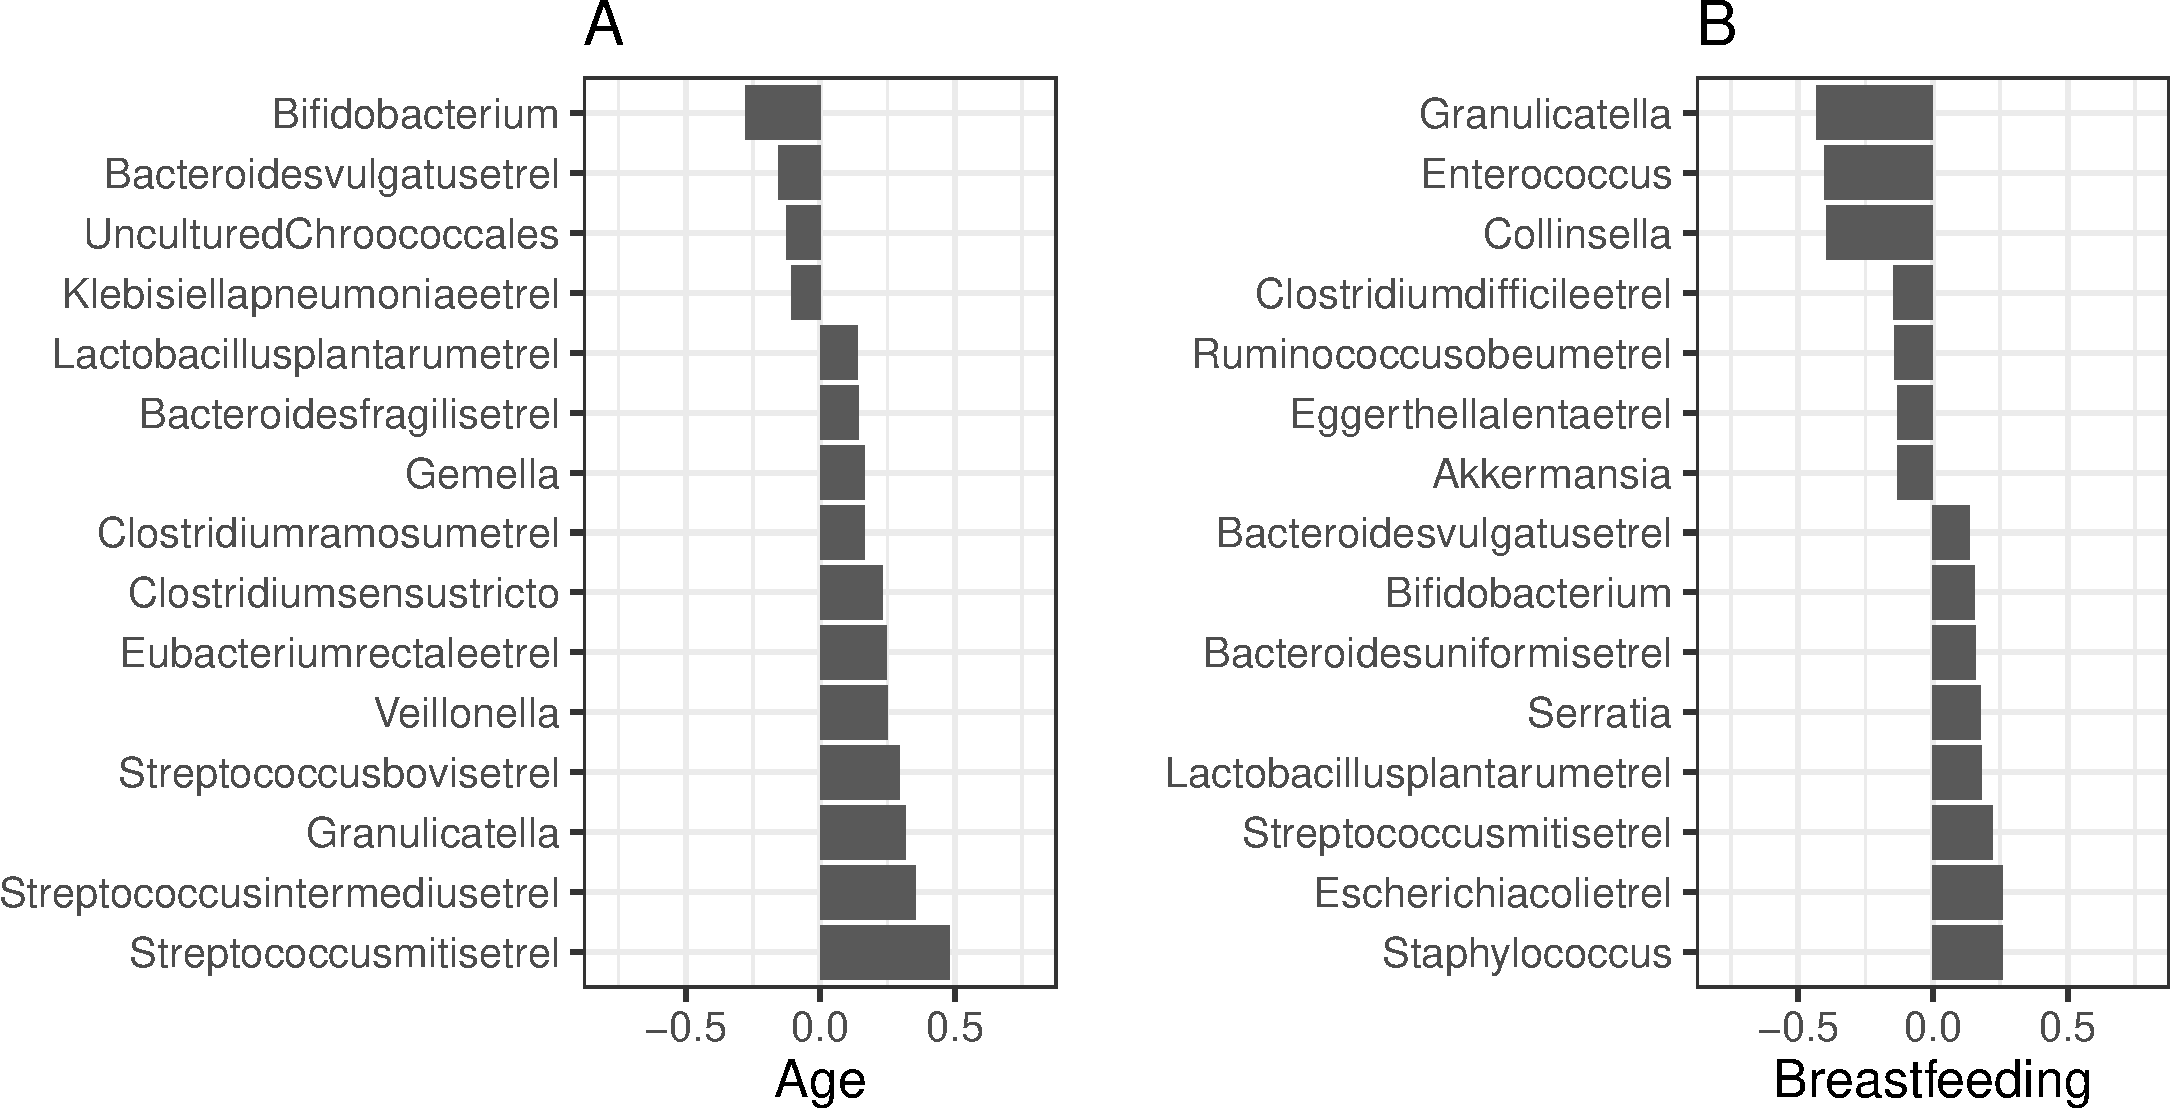
\includegraphics{index_files/figure-latex/unnamed-chunk-10-1.pdf}
\caption{\label{fig:unnamed-chunk-10}Top Taxa that differ most as a function
of each predictor.}
\end{figure}

\subsubsection{3.3 Differential abundance with Bayesian
GLM}\label{differential-abundance-with-bayesian-glm}

We modeled clr-transformed bacterial abundance using the generalized
Gaussian distribution with constant variance \(\sigma\) and skewness
parameter \(\alpha\). The parameter \(\mu\) is modeled as a linear
function of the predictors \enquote{cc}, \enquote{time},
\enquote{breastfeeding} and \enquote{age}. Note that \(\mu\) does only
represent the mean if \(\alpha = 0\). Figures x-x show the arithmetric
means of the posterior distribution of the differences in \(\mu\)
between the groups with 95\% highest probability density interval. Only
those genera are shown that were different with high certainty in at
least one comparison. Figure x shows the comparison between CC and HOME
for each time point whereas figure x shows the difference between PRE
and POST within each group. There are similar trends in all comparisons
for \emph{Streptococcus intermedius et rel}, \emph{Streptococcus mitis
et rel} and \emph{Granulicatella}. However it seems as if this change is
stronger in the CC group since here these genera are decreasing over
time with higher certainty (\(\geq 95\) \%). Since we are looking at
clr-transformed abundances it is also possible that all other genera
increased relative to the above mentioned genera (\textbf{at Gerben: you
have more experience with interpreting clr-transformed abundances. I am
still reading about this so please edit this so that we make those
interpretation we can make}).

\begin{figure}
\centering
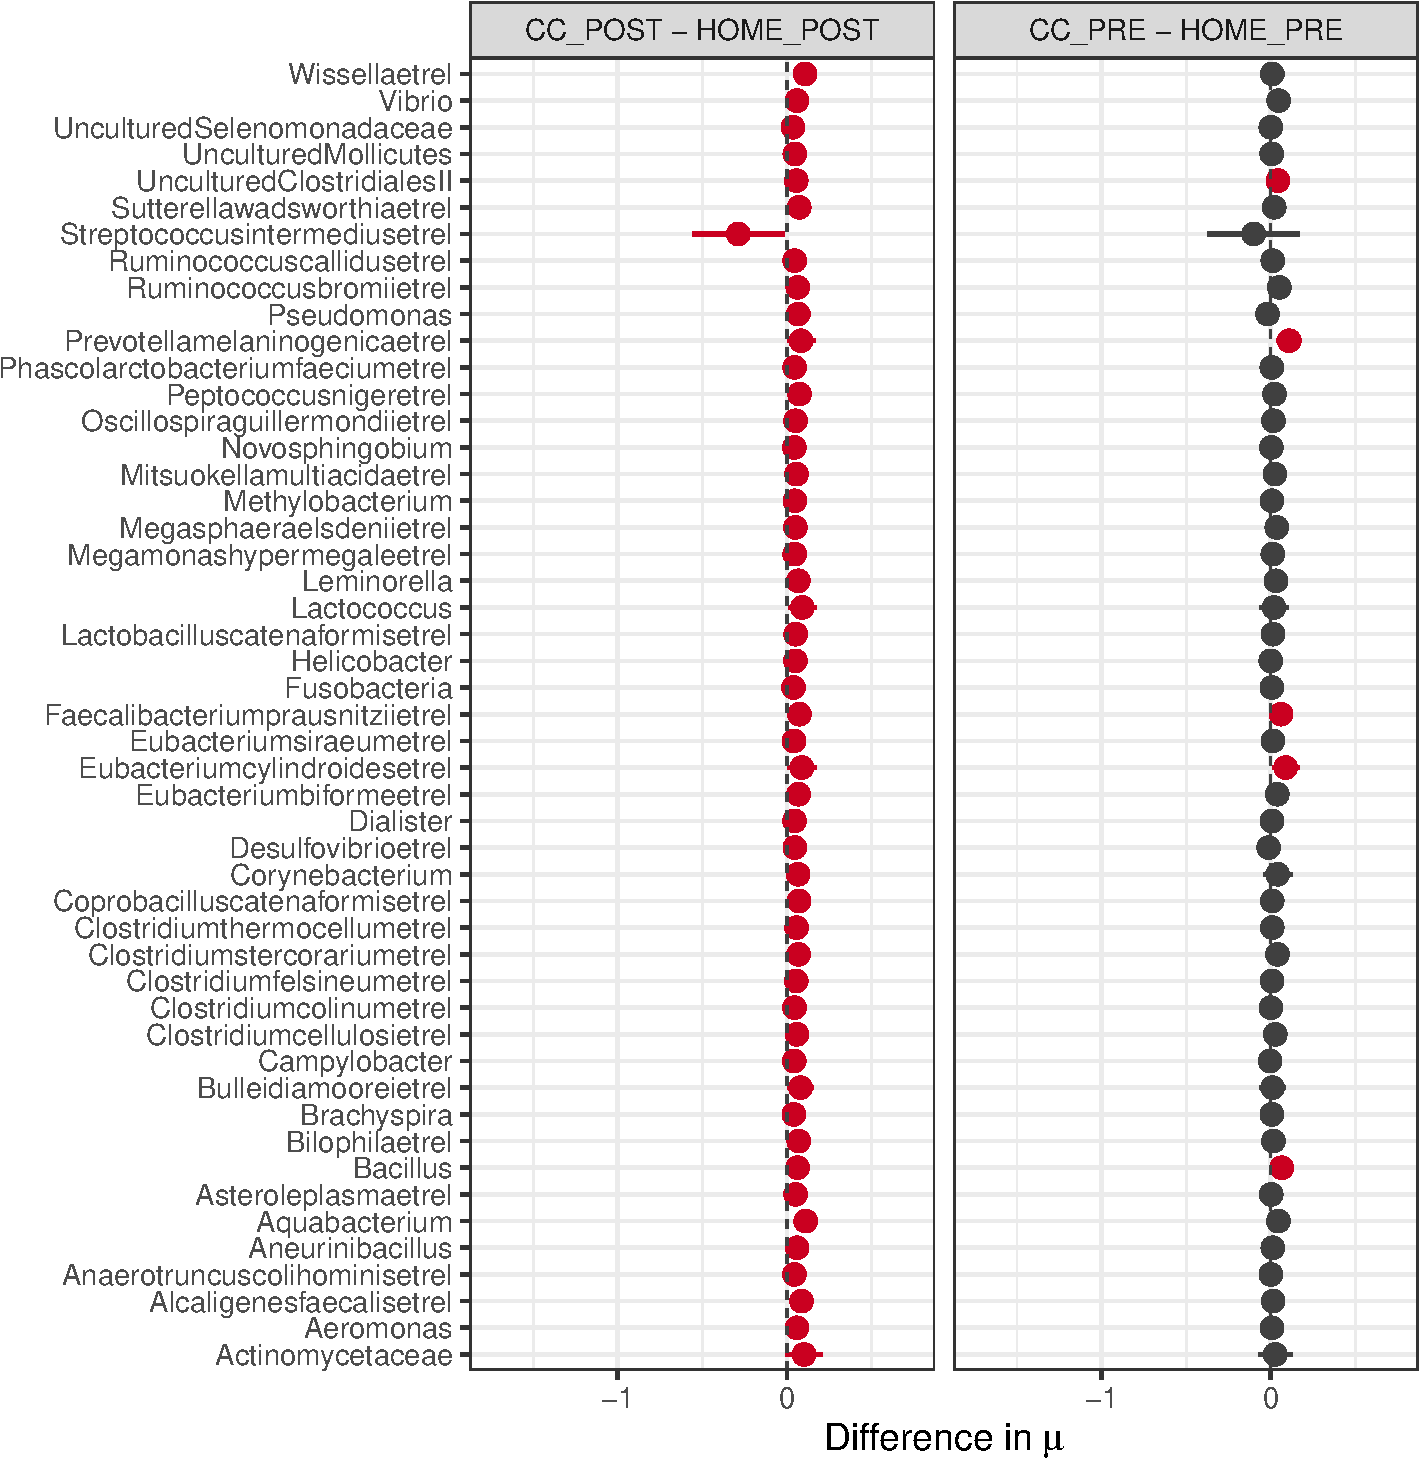
\includegraphics{index_files/figure-latex/unnamed-chunk-11-1.pdf}
\caption{\label{fig:unnamed-chunk-11}Posterior distribution of the
difference in mu between CC and HOME.}
\end{figure}

\begin{figure}
\centering
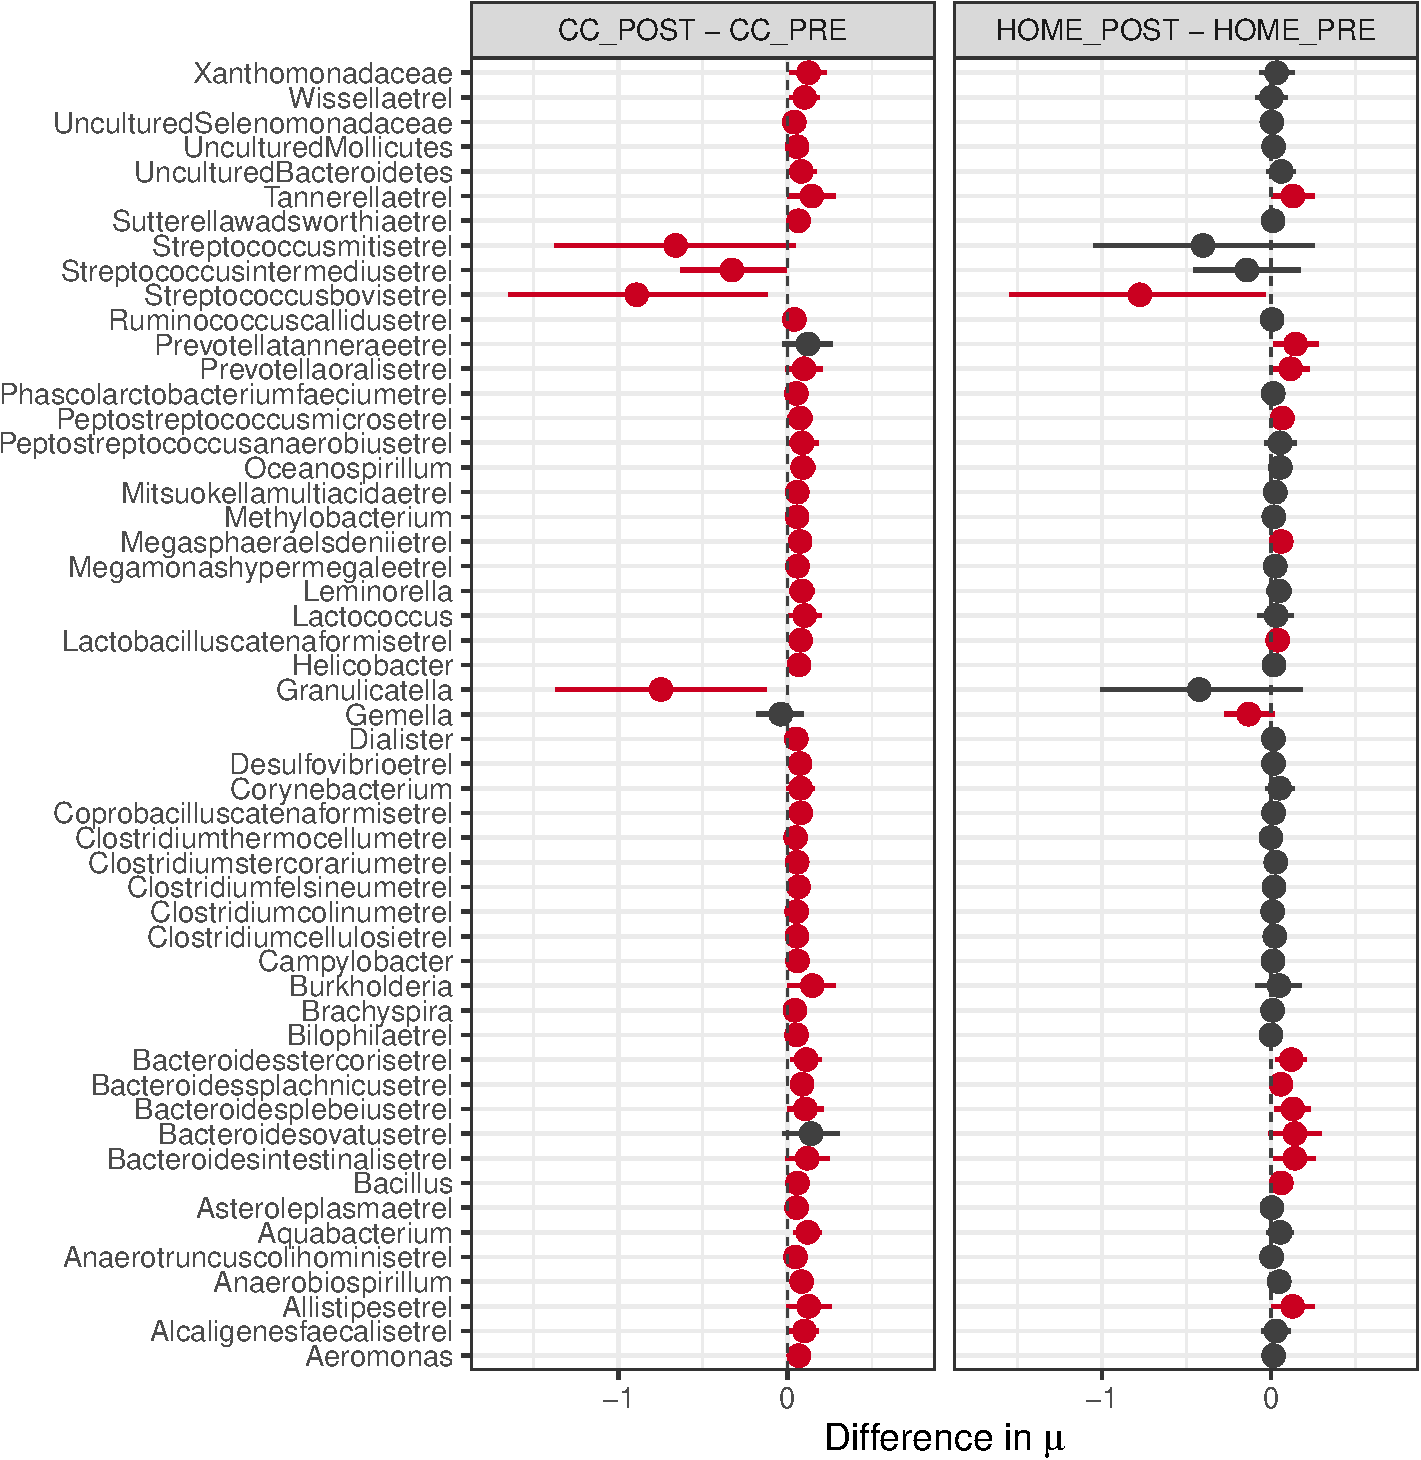
\includegraphics{index_files/figure-latex/unnamed-chunk-12-1.pdf}
\caption{\label{fig:unnamed-chunk-12}Posterior distribution of the
difference in mu within CC and HOME.}
\end{figure}

\subsubsection{3.4 Alpha diversity with
Bayesian}\label{alpha-diversity-with-bayesian}

\textbf{Should we maybe only report one? I reported three only be
because the results are slightly different depending on the index)}

Alpha diversity (Shannon) was calculated using the \emph{microbiome}
package before the clr-transformation. Alpha-diversity was assumed to be
Gaussian distributed with constant variance \(\sigma\) and skewness
parameter \(\alpha\). Table x shows the estimated difference in the
parameter \(\mu\) of the generalized Gaussian distribution between
groups as well as the estimated \(\alpha\) and \(\sigma\). There was no
difference in alpha diversity within the HOME group or between HOME and
CC before childcare entrance. Comparing \(\mu\) within CC or between
HOME and CC after entrance, we see that diversity is lower in the CC
group with high certainty suggesting that CC leads to a decrease in
alpha diversity. Figure 3 shows alpha diversity for each subject for
each subgroup. It furthermore shows the highest probability density
interval of \(\mu\) for each group. We see that \(\mu\) was highest in
the CC group before entrance and lowest of all groups after CC
attendance. However, we see large individual variation within each group
and the difference in \(\mu\) is small (table x).

\begin{table}[tbp]
\begin{center}
\begin{threeparttable}
\caption{\label{tab:unnamed-chunk-13}Estimated model parameters alpha diversity.}
\begin{tabular}{llll}
\toprule
Parameter & \multicolumn{1}{c}{Mean} & \multicolumn{1}{c}{95\% HPDI} & \multicolumn{1}{c}{P(Parameter < 0)}\\
\midrule
Alpha & -1.60 & [-6.22, 2.21] & 0.75\\
CC\_POST - CC\_PRE & -0.29 & [-0.52, -0.07] & 0.99\\
CC\_POST - HOME\_POST & -0.22 & [-0.4, -0.03] & 0.99\\
CC\_PRE - HOME\_PRE & 0.05 & [-0.14, 0.23] & 0.31\\
HOME\_POST - HOME\_PRE & -0.03 & [-0.25, 0.19] & 0.60\\
Sigma & 0.33 & [0.27, 0.39] & 0.00\\
\bottomrule
\end{tabular}
\end{threeparttable}
\end{center}
\end{table}

\begin{figure}
\centering
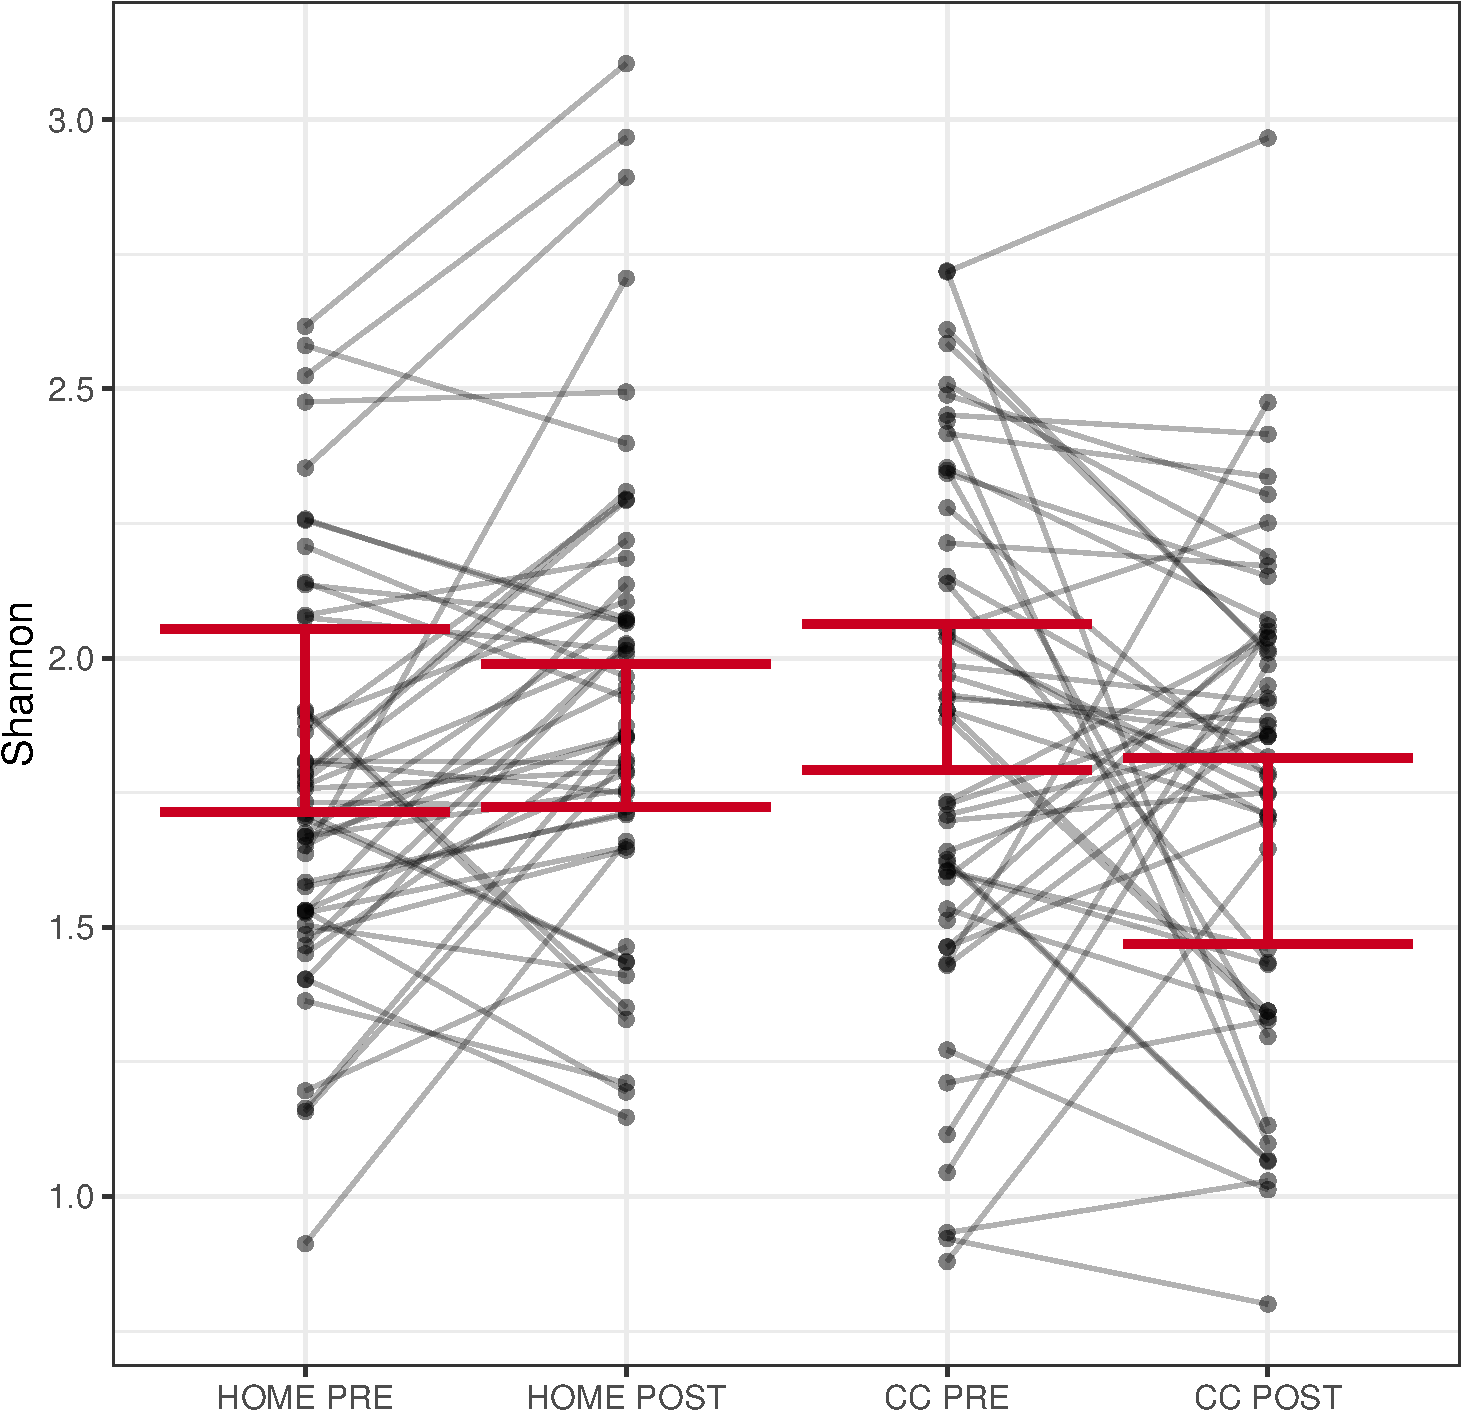
\includegraphics{index_files/figure-latex/unnamed-chunk-14-1.pdf}
\caption{\label{fig:unnamed-chunk-14}Observed values of alpha-diversity,
individual paths and posterior distribution of mu.}
\end{figure}

\subsection{3.4 Random Forest}\label{random-forest}

RF is a tree based ensemble learning method that is well suited for
classification based on microbial abundances of samples
({\textbf{???}}). We randomly selected 80\% of the collected samples
that constituted the training data set. We first tuned the RF models
based on out-of-bag error. Node splitting was based on the gini
criterion. Then we evaluated whether we can correctly classify CC based
on 130 genus abundances using the hold out set. According to our
hypotheses, we would expect to be able to classify whether an infant in
the test data set belongs to the CC group at T1. In contrast, at T0 we
would expect prediction accuracy to be lower since there should be no
differences between CC and HOME. However, neither the T0 model, nor the
model for T1 achieved a higher prediction accuracy than 0.5 suggesting
that there was no systematic effect of childcare entrance on microbiota
composition.

\newpage

\newpage

\section{References}\label{references}

\begingroup
\setlength{\parindent}{-0.5in} \setlength{\leftskip}{0.5in}

\hypertarget{refs}{}

\endgroup

\clearpage

\renewcommand{\listfigurename}{Figure captions}

\listoffigures

\clearpage

\renewcommand{\listtablename}{Table captions}

\listoftables


\end{document}
